\documentclass[tikz]{standalone}

\usetikzlibrary{shapes, decorations, arrows ,calc, arrows.meta,
                fit, positioning, automata, shapes.geometric, patterns}

\usepackage{tikz}

\begin{document}

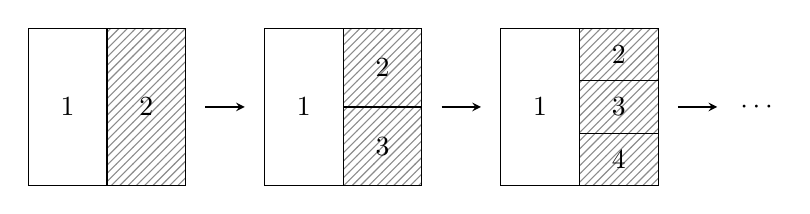
\begin{tikzpicture}
\filldraw[pattern color=gray, pattern=north east lines, opacity=0.9] (0,-1) -- (0,1) -- (1,1) -- (1,-1) -- cycle;
\node[] at (-0.5, 0) {1};
\node[] at (0.5, 0) {2};
\draw (-1,1) -- (1,1);
\draw (-1,-1) -- (1,-1);
\draw (-1,-1) -- (-1,1);
\draw (1,-1) -- (1,1);
\draw (0,-1) -- (0,1);

\filldraw[pattern color=gray, pattern=north east lines, opacity=0.9] (3,-1) -- (3,1) -- (4,1) -- (4,-1) -- cycle;
\node[] at (2.5, 0) {1};
\node[] at (3.5, 0.5) {2};
\node[] at (3.5, -0.5) {3};
\draw (2,1) -- (4,1);
\draw (2,-1) -- (4,-1);
\draw (2,-1) -- (2,1);
\draw (4,-1) -- (4,1);
\draw (3,-1) -- (3,1);
\draw (3,0) -- (4,0);

\filldraw[pattern color=gray, pattern=north east lines, opacity=0.9] (6,-1) -- (6,1) -- (7,1) -- (7,-1) -- cycle;
\node[] at (5.5, 0) {1};
\node[] at (6.5, 0.666) {2};
\node[] at (6.5, 0) {3};
\node[] at (6.5, -0.666) {4};
\draw (5,1) -- (7,1);
\draw (5,-1) -- (7,-1);
\draw (5,-1) -- (5,1);
\draw (7,-1) -- (7,1);
\draw (6,-1) -- (6,1);
\draw (6,-0.333) -- (7,-0.333);
\draw (6,0.333) -- (7,0.333);

\draw [->,>=stealth] (1.25,0) -- (1.75,0);
\draw [->,>=stealth] (4.25,0) -- (4.75,0);
\draw [->,>=stealth] (7.25,0) -- (7.75,0);

\node[] at (8.25, 0) {$\cdots$};
\end{tikzpicture}

\end{document}
